\chapter{Dimensional Dependence of Optical Transition Rates} \label{RM}
 
%\section{Time-dependent Perturbation Theory} \label{dust_seds}

\subsection{Fermi's Golden Rule} \label{dust_corrections}

When the semiconductor illuminated by light, the interaction between the photons and the electrons in the semiconductor can be described by the Hamiltonian:

\begin{equation}
  \HAM = \frac{1}{2m_0}{(\bm{p}-e\bm{A})}^2+V(\bm{r})
\end{equation}

where $m_0$ is the free electron mass, $e=-|e|$ for electrons, $\bm{A}$ is the vector potential accounting for the presence of the electromagnetic field, and $V(\bm{r})$ is the periodic crystal potential.

The Hamiltonian can be expanded into


\begin{eqnarray}
  & \HAM = \frac{1}{2m_0}{(\bm{p}-e\bm{A})}^2+V(\bm{r})
  &  \approx \HAM_0+\HAM^\prime
\end{eqnarray}

where $\HAM_0$ is the unperturbed Hamiltonian and ${\HAM}^\prime$ is considered as a perturbation due to light

\begin{equation}
\HAM_0=\frac{{\bm{p}}^2}{2m_0}+V(\bm{r})
\end{equation}

\begin{equation}
  \HAM^\prime=-\frac{e}{m_0}\bm{A}\bm{p}
\end{equation}

and consider the coulomb gauge has been used.

\begin{equation}
  \nabla\cdot\bm{A}=0
\end{equation}

noting that $\bm{p}=(\hbar/i)\nabla$, so $\bm{p}\cdot\bm{A}=(\frac{\hbar}{i})\nabla\cdot\bm{A}=\bm{A}\cdot\bm{p}$. And since we know $\bm{p}\approx\hbar{k}\approx\hbar\frac{\pi}{a}$, and $a$ is the lattice constant, usually have a value of $5\mathring{A}$, so $|e\bm{A}|\ll|\bm{p}|$, then we can drop the last term $\frac{e^2{\bm{A}}^2}{2m_0}$, because it is much smaller than the terms linear in $\bm{A}$.

Assume the vector potential for the optical electric field of the form

\begin{eqnarray}
  & \bm{A} = \hat{e}\bm{A}_0\cos{k_{op}\cdot\bm{r}-\omega{t}}
  & = \hat{e}\frac{A_0}{2}e^{ik_{op}\cdot\bm{r}}e^{-i\omega{t}} + \hat{e}\frac{A_0}{2}e^{-ik_{op}\cdot\bm{r}}e^{i\omega{t}}
\end{eqnarray}

where $\bm{k_{op}}$ is the wave vector, $\omega$ is the optical angular frequency, and $\hat{e}$ is a unit vector in the direction of the optical electric field, we have

\begin{equation}
  \bm{E}(\bm{r},t) = -\frac{\partial\bm{A}}{\partial{t}}= -\hat{e}\omega{\bm_{A}}_0\sin{\bm{k_{op}}\cdot\bm{r}-\omega{t}}
\end{equation}

\begin{equation}
  \bm{H}\left( \bm{r,}t \right) = \frac{1}{\mu}\nabla \times \bm{A} = - \frac{1}{\mu}\bm{k_{\bm{\text{op}}}}\bm{\times}\hat{e}A_{0}\sin\left( \bm{k}_{\bm{\text{op}}} \cdot \bm{r} - \omega t \right)
\end{equation}

where we have used the fact that the scalar potential \(\varphi\)
vanishes (\(\rho = 0\)) for the optical field, and \(\mu = \mu_{0}\), the
permeability of the free space. The Poynting vector for the power
intensity \((W/\text{cm}^{2})\) is given by

\begin{equation}
  \bm{P}\left( \bm{r,}t \right) = \bm{E}\left( \bm{r,}t \right) \times \bm{H}\left( \bm{r,}t \right) = \hat{k}\bm{k}_{\bm{\text{op}}}\frac{\omega{A_{0}}^{2}}{\mu}\operatorname{}\left( \bm{k}_{\bm{\text{op}}} \cdot \bm{r} - \omega t \right)
\end{equation}

which is pointing along the direction of wave propagation
\(\bm{k}_{\bm{\text{op}}}\). The time average of the Poynting
flux is simply

\begin{eqnarray}
& \bm{P} = \left| \bm{P}\left( \bm{r,}t \right) \right| = \frac{\omega{A_{0}}^{2}}{2\mu}\bm{k}_{\bm{\text{op}}} \nonumber \\
& = \frac{\omega^{2}{A_{0}}^{2}n_{r}}{2\mu{c}} \nonumber \\
& = \frac{\omega^{2}{A_{0}}^{2}n_{r}\sqrt{\mu_{0}\varepsilon_{0}}}{2\mu_{0}} \nonumber \\
& = \frac{\omega^{2}{A_{0}}^{2}n_{r}\sqrt{\varepsilon_{0}}}{2\sqrt{\mu_{0}}} \nonumber \\
& = \frac{\omega^{2}{A_{0}}^{2}n_{r}\sqrt{\varepsilon_{0}}\sqrt{\varepsilon_{0}}}{2\sqrt{\mu_{0}}\sqrt{\varepsilon_{0}}} \nonumber \\
& = \frac{\omega^{2}{A_{0}}^{2}n_{r}\varepsilon_{0}c}{2}
\end{eqnarray}

Noting the time average of the \(\sin^{2}()\) function is
\(\frac{1}{2}\) and
\(\bm{k}_{\bm{\text{op}}}\bm{=}\omega\sqrt{\mu\varepsilon_{0}} = \frac{\omega}{\nu} = \frac{\omega}{\frac{c}{n_{r}}}\),
\(c = \frac{1}{\sqrt{\mu_{0}\varepsilon_{0}}}\)

The interaction Hamiltonian

\begin{eqnarray}
  & \HAM^{\bm{'}}\left( \bm{r,}t \right)\bm{=} - \frac{e}{m_{0}}\bm{\ A(r,}t\bm{) \cdot p} \nonumber \\
  & \bm{=}\HAM^{\bm{'}}\left( \bm{r} \right)\bm{e}^{\bm{- i\omega t}}\bm{+}\HAM^{\bm{' +}}\left( \bm{r} \right)\bm{e}^{\bm{+ i\omega t}}
\end{eqnarray}

where

\begin{equation}
\HAM^{\bm{'}}\left( \bm{r} \right)\bm{=} - \frac{eA_{0}\bm{e}^{\bm{i}\bm{k}_{\bm{\text{op}}}\bm{\cdot r}}}{2m_{0}}\bm{\  \cdot}\hat{e}\bm{\cdot p}
\end{equation}

The superscript ``+'' means the Hermitian adjoint operator.

The transition rate for the absorption of a photon:

If the electron is at state a initially. And assume \(E_{b} > E_{a}\)

\begin{equation}
W_{\text{abs}} = \frac{2\pi}{\hbar}\left| \left\langle b \middle| \HAM^{\bm{'}}\left( \bm{r} \right) \middle| a \right\rangle \right|^{2}\delta(E_{b} - E_{a} - \hbar\omega)
\end{equation}

The total upward transition rate per unit volume
\((s^{- 1}\text{cm}^{- 3})\) in the crystal taking into account the
probability that state a is occupied and state b is empty:

\begin{equation}
R_{a \rightarrow b} = \frac{2}{V}\sum_{\bm{k}_{a}}^{}{\sum_{\bm{k}_{b}}^{}\frac{2\pi}{\hbar}}\left| {\HAM^{'}}_{\text{ba}} \right|^{2}\delta(E_{b} - E_{a} - \hbar\omega)f_{a}(1 - f_{b})
\end{equation}

where we sum over the initial and final states and assume that the
Fermi-Dirac distribution \(f_{a}\) is the probability that the state a
is occupied. A similar expression holds for \(f_{b}\) with \(E_{a}\)
replaced by \(E_{b}\), and \(\left( 1 - f_{b} \right)\) is the
probability that the state b is empty. The prefactor 2 takes into
account the sum over spins, and the matrix element
\({\HAM^{'}}_{\text{ba}}\) is given by \textbf{Fermi's Golden Rule}

\begin{equation}
{\HAM^{'}}_{\text{ba}} \equiv \left| \left\langle b \middle| \HAM^{\bm{'}}\left( \bm{r} \right) \middle| a \right\rangle \right| = \int_{}^{}{\Psi_{b}^{*}\left( \bm{r} \right)H^{'}\left( \bm{r},t \right)\Psi_{a}\left( \bm{r} \right)d^{3}\bm{r}}
\end{equation}

Similarly, the transition rate for the emission of a photon if an
electron is initially at state b is

\begin{equation}
W_{\text{ems}} = \frac{2\pi}{\hbar}\left| \left\langle a \middle| \HAM^{\bm{'}}\left( \bm{r} \right) \middle| b \right\rangle \right|^{2}\delta(E_{a} - E_{b} + \hbar\omega)
\end{equation}

The downward transition rate per unit volume
\((s^{- 1}\text{cm}^{- 3})\) is

\begin{equation}
R_{b \rightarrow a} = \frac{2}{V}\sum_{\bm{k}_{a}}^{}{\sum_{\bm{k}_{b}}^{}\frac{2\pi}{\hbar}}\left| {\HAM^{' +}}_{\text{ab}} \right|^{2}\delta(E_{a} - E_{b} + \hbar\omega)f_{b}(1 - f_{a})
\end{equation}

Using the even property of the delta function,
\(\delta\left( - x \right) = \delta\left( x \right)\), and
\({\HAM^{'}}_{\text{ba}} = {\HAM^{' +}}_{\text{ab}}\), the net upward
transition rate per unit volume can be written as

\begin{equation}
R = R_{a \rightarrow b} - R_{b \rightarrow a} = \frac{2}{V}\sum_{\bm{k}_{a}}^{}{\sum_{\bm{k}_{b}}^{}\frac{2\pi}{\hbar}}\left| {\HAM^{'}}_{\text{ba}} \right|^{2}\delta(E_{b} - E_{a} - \hbar\omega)(f_{a} - f_{b})
\end{equation}

The absorption coefficient \(\alpha(1/cm)\) in the crystal is the
fraction of photons absorbed per unit distance:

\begin{equation}
\alpha = \frac{\text{Number\ of\ photons\ absorbed\ per\ second\ per\ unit\ volume}}{\text{Number\ of\ injected\ photons\ per\ second\ per\ unit\ area}}
\end{equation}

The injected number of photons per second per unit area is the optical
intensity \(P(W/\text{cm}^{2})\) divided by the energy of a photon
\(\hbar\omega\):

\begin{equation}
\alpha\left( \hbar\omega \right) = \frac{R}{\frac{P}{\hbar\omega}} = \frac{\hbar\omega}{(\frac{n_{r}c\epsilon_{0}\omega^{2}A_{0}^{2}}{2})}R
\end{equation}

Using the long wavelength approximation that
\(\bm{A}\left( \bm{r} \right) = \bm{A}e^{i\bm{k}_{\bm{\text{op}}}\bm{\cdot}r}\bm{\approx A}\),
we find that the matrix element can be written in terms of the momentum
matrix element

\begin{equation}
{\HAM^{'}}_{\text{ba}} = - \frac{e}{m_{0}}\bm{\ A \cdot}\left\langle b \middle| \bm{p} \middle| a \right\rangle\bm{=}\frac{eA_{0}}{2m_{0}}\bm{\  \cdot}\hat{e}\bm{\cdot}\bm{p}_{\text{ba}}
\end{equation}

The absorption coefficient becomes

\begin{eqnarray}
  & \alpha\left( \hbar\omega \right) = C_{0}\frac{2}{V}\sum_{\bm{k}_{a}}^{}{\sum_{\bm{k}_{b}}^{}\left| \hat{e}\bm{\cdot}\bm{p}_{\text{ba}} \right|^{2}}\delta(E_{b} - E_{a} - \hbar\omega)(f_{a} - f_{b}) \nonumber \\
  & C_{0} = \frac{\pi e^{2}}{n_{r}\varepsilon_{0}cm_{0}^{2}\omega}
\end{eqnarray}


\section{Interband Absorption for a Bulk
Semiconductor}\label{interband-absorption-for-a-bulk-semiconductor}

Evaluate the optical matrix element:

\begin{equation}
{\HAM^{'}}_{\text{ba}} = \bm{\ }\left\langle b \middle| - \frac{e\bm{A(r)}}{m_{0}}\bm{\cdot p} \middle| a \right\rangle
\end{equation}

The vector potential for the optical field is

\begin{equation}
\bm{A}\left( \bm{r} \right)\bm{= A}{\cdot e}^{i\bm{k}_{\bm{\text{op}}} \cdot r} = \frac{\hat{e}A_{0}}{2}e^{i\bm{k}_{\bm{\text{op}}} \cdot r}
\end{equation}

The Bloch functions for electrons in the valence band \(E_{a}\) and the
conduction band \(E_{b}\) are:

\begin{equation}
\Psi_{a}\left( \bm{r} \right) = u_{v}(\bm{r})\frac{e^{i\bm{k}_{\bm{v}} \cdot r}}{\sqrt{V}}
\end{equation}

\begin{equation}
\Psi_{b}\left( \bm{r} \right) = u_{c}(\bm{r})\frac{e^{i\bm{k}_{\bm{c}} \cdot r}}{\sqrt{V}}
\end{equation}

where \(u_{v}(\bm{r})\) and \(u_{c}(\bm{r})\) are the periodic
parts of the Bloch functions, and the remainders are the envelope
functions (plane waves) for a free electron. The momentum matrix element
is derived from

\begin{eqnarray}
  & {\HAM^{'}}_{\text{ba}} = - \frac{eA_{0}}{2m_{0}}\bm{\ }\hat{e}\bm{\cdot}\int_{}^{}{\Psi_{b}^{*}e^{i\bm{k}_{\bm{\text{op}}}\bm{\cdot}r}\bm{p}\Psi_{a}d^{3}\bm{r}} \nonumber \\
  & = - \frac{eA_{0}}{2m_{0}}\bm{\ }\hat{e}\bm{\cdot}\int_{}^{}{u_{c}(\bm{r})e^{i\bm{k}_{\bm{c}} \cdot r}e^{i\bm{k}_{\bm{\text{op}}}\bm{\cdot}r}\left\lbrack \left( \frac{\hbar}{i}\nabla u_{v}(\bm{r}) \right)e^{i\bm{k}_{\bm{v}} \cdot r} + \hbar\bm{k}_{\bm{v}}u_{v}(\bm{r})e^{i\bm{k}_{\bm{v}} \cdot r} \right\rbrack\frac{d^{3}\bm{r}}{V}} \nonumber \\
  & \approx - \frac{eA_{0}}{2m_{0}}\bm{\ }\hat{e}\bm{\cdot}\int_{\Omega}^{}{{u_{c}}^{*}(\bm{r}){\frac{\hbar}{i}\nabla u}_{v}(\bm{r})}\frac{d^{3}\bm{r}}{\Omega}\int_{V}^{}e^{i{\bm{( -}\bm{k}_{\bm{c}}\bm{+}\bm{k}_{\bm{\text{op}}}\bm{+ k}}_{\bm{v}}) \cdot r}\frac{d^{3}\bm{r}}{V} \nonumber \\
  & = - \frac{eA_{0}}{2m_{0}}\bm{\ }\hat{e}\bm{\cdot}\bm{p}_{\text{cv}}\delta_{{\bm{k}_{\bm{c,}}\bm{k}_{\bm{\text{op}}}\bm{+ k}}_{\bm{v}}}
\end{eqnarray}

\begin{equation}
\bm{p}_{\text{cv}}\bm{=}\int_{\Omega}^{}{{u_{c}}^{*}(\bm{r}){\frac{\hbar}{i}\nabla u}_{v}(\bm{r})}\frac{d^{3}\bm{r}}{\Omega}
\end{equation}

where we noted that
\(\left\lbrack {u_{c}}^{*}(\bm{r})\frac{\hbar}{i}\nabla u_{v}(\bm{r}) \right\rbrack\)
and
\(\left\lbrack {u_{c}}^{*}(\bm{r})u_{v}(\bm{r}) \right\rbrack\)
are periodic functions with the period of a unit cell, whereas the
envelope functions are slowly varying functions over a unit cell.
Therefore, the integral over \(d^{3}\bm{r}\) can be separated into
the product of two integrals, one over the unit cell \(\Omega\) for the
periodic part, and the other over the slowly varying part. In another
word, we use the approximation:

\begin{equation}
\int_{V}^{}\left\lbrack {u_{c}}^{*}\left( \bm{r} \right){\frac{\hbar}{i}\nabla u}_{v}\left( \bm{r} \right) \right\rbrack F(\bm{r})d^{3}\bm{r \approx}\int_{V}^{}{F(\bm{r})}d^{3}\bm{r}\int_{\Omega}^{}{{u_{c}}^{*}(\bm{r}){\frac{\hbar}{i}\nabla u}_{v}(\bm{r})}\frac{d^{3}\bm{r}}{\Omega}
\end{equation}

where \(F(\bm{r})\) is slowly varying over a unit cell, and we have
used the periodic property of the Bloch periodic functions

\begin{equation}
{u_{c}}^{*}\left( \bm{r} \right){\frac{\hbar}{i}\nabla u}_{v}\left( \bm{r} \right) = \sum_{\bm{G}}^{}{\bm{C}_{\bm{G}}e^{i\bm{G} \cdot r}}
\end{equation}

where the vectors \(\bm{G}^{\bm{'}}s\) are the reciprocal
lattice vectors. Because \(F\left( \bm{r} \right)\) is slowly
varying over a unit cell, we may approximate
\(F\left( \bm{r + R} \right) = F\left( \bm{R} \right)\) and put
it outside of the integral over a unit cell. Here the \emph{\textbf{R}}s
are the lattice vectors, and
\(e^{i\bm{G} \cdot \bm{R}} = 1\).\(\omega\) is the volume
of a unit cell. Note that the orthogonal property

\begin{eqnarray}
  & \int_{\Omega}^{}{{u_{c}}^{*}u_{v}d^{3}\bm{r} = 0}, \nonumber \\
  & \frac{1}{\Omega}\int_{\Omega}^{}{{u_{c}}^{*}u_{c}d^{3}\bm{r} = \frac{1}{\Omega}\int_{\Omega}^{}{{u_{v}}^{*}u_{v}d^{3}\bm{r} = 1}}
\end{eqnarray}

From the matrix element, we see the momentum conservation

\begin{equation}
\hbar\bm{k}_{c} = \hbar\bm{k}_{v} + \hbar\bm{k}_{\text{op}}
\end{equation}

is obeyed. The electron at the final state has its crystal momentum
\(\hbar\bm{k}_{\text{c\ }}\)equal to its initial momentum\(\hbar\bm{k}_{v}\)
plus the photon momentum\(\hbar\bm{k}_{\text{op}}\). Because
\(\bm{k}_{\text{op}}\sim\frac{2\pi}{\lambda_{0}}\), and the magnitudes
\(\bm{k}_{\text{c\ }},\bm{k}_{\text{v\ }}\) are of the order\(\
\frac{2\pi}{a_{0}}\), where \(a_{0}\ \)is the lattice constant of the
semiconductors, which is typically of the order $5.5\mathring{A}$  and is much
smaller than we may ignore \(\bm{k}_{\text{op}}\) and obtain

\begin{equation}
{\HAM^{'}}_{\text{ba}} \approx - \frac{eA_{0}}{2m_{0}}\bm{\ }\hat{e}\bm{\cdot}\bm{p}_{\text{cv}}\delta_{{\bm{k}_{\bm{c,}}\bm{k}}_{\bm{v}}}
\end{equation}

which is the \textbf{K}-selection Rule.

\begin{enumerate}
\def\labelenumi{\arabic{enumi})}
\item
  Interband momentum matrix element \(\bm{p}_{\text{cv}}\) depend
  only on the periodic parts of the Bloch functions
  (\(u_{c}\text{\ and\ }u_{v}\)),
\item
  The original optical momentum matrix element
  \(\bm{p}_{\text{ab}}\), depends on the full wave functions (i.e.
  including the envelope function).
\end{enumerate}

Using the \textbf{K}-selection rule in the matrix element, we find that
the absorption coefficient for a bulk semiconductor is

\begin{eqnarray}
& \alpha\left( \hbar\omega \right) = C_{0}\frac{2}{V}\sum_{\bm{k}_{a}}^{}{\sum_{\bm{k}_{b}}^{}\left| \hat{e}\bm{\cdot}\bm{p}_{\text{cv}} \right|^{2}}\delta(E_{c} - E_{v} - \hbar\omega)(f_{v} - f_{c}) \nonumber \\
  & C_{0} = \frac{\pi e^{2}}{n_{r}\varepsilon_{0}cm_{0}^{2}\omega}
\end{eqnarray}

where the Fermi-Dirac distributions for the electrons in the valence
bend and in the conduction band are, respectively.

\begin{equation}
f_{v}\left( k \right) = \frac{1}{1 + e^{\frac{(E_{v}\left( k \right) - F_{v})}{\text{KT}}}}
,
f_{c}\left( k \right) = \frac{1}{1 + e^{\frac{(E_{c}\left( k \right) - F_{c})}{\text{KT}}}}
\end{equation}

Assume:

\begin{enumerate}
\def\labelenumi{\arabic{enumi})}
\item
  \(\bm{k}_{\text{c\ }} = \bm{k}_{\text{v\ }} = \bm{k}\)\textbf{,}
  \(F_{v} = F_{c} = E_{F}\) (thermal equilibrium)
\item
  \(f_{v} = 1\ and\ f_{c} = 0\)
\item
  \(\left| \hat{e}\bm{\cdot}\bm{p}_{\text{cv}} \right|^{2}\)
  is independent of \(\bm{k}\) and denote the absorption spectrum at
  thermal equilibrium.
\end{enumerate}

\begin{equation}
\alpha\left( \hbar\omega \right) = C_{0}\left| \hat{e}\bm{\cdot}\bm{p}_{\text{cv}} \right|^{2}\int_{}^{}\frac{2d^{3}\bm{k}}{\left( 2\pi \right)^{3}}\delta(E_{g} + \frac{\hbar^{2}\bm{k}^{\bm{2}}}{2m_{r}^{*}} - \hbar\omega)
\end{equation}

where used the reduced effective mass \(m_{r}^{*}\)

\begin{eqnarray}
  \begin{aligned}
  & E_{c} = E_{g} + \frac{\hbar^{2}\bm{k}^{\bm{2}}}{2m_{r}^{*}}
  & E_{v} = - \frac{\hbar^{2}\bm{k}^{\bm{2}}}{2m_{r}^{*}} \nonumber \\
  & \frac{1}{m_{r}^{*}} = \frac{1}{m_{e}^{*}} + \frac{1}{m_{h}^{*}} 
  \end{aligned}
\end{eqnarray}

Here all energies are measured from the top of the valence band.
Therefore, both \(E_{c}\text{\ and\ }F_{c}\) contain the band-gap energy
\(E_{g}\). Let

\begin{eqnarray}
  & X = E_{g} + E - \hbar\omega
  & E = \frac{\hbar^{2}\bm{k}^{\bm{2}}}{2m_{r}^{*}}
\end{eqnarray}

we find, by a change of variables, the integration can be carried out
with the contribution at \(X = 0,\ and\ E = {\hbar\omega - E}_{g}\)

\begin{eqnarray}
  & \alpha\left( \hbar\omega \right) = C_{0}\left| \hat{e}\bm{\cdot}\bm{p}_{\text{cv}} \right|^{2}\rho_{r}\left( {\hbar\omega - E}_{g} \right)  \\
  & \rho_{r}\left( {\hbar\omega - E}_{g} \right) = \frac{1}{2\pi^{2}}{(\frac{2m_{r}^{*}}{\hbar^{2}})}^{\frac{3}{2}}\left( {\hbar\omega - E}_{g} \right)^{\frac{1}{2}}
\end{eqnarray}

Therefore, the absorption coefficient depends on the momentum matrix
element and the joint optical density of states. Below the band-gap
energy \(E_{g}\), the absorption does not occur because the photons see
a forbidden band gap.

\section{Interband Absorption and Gain in A Quantum
Well}\label{interband-absorption-and-gain-in-a-quantum-well}

The central cell functions in the quantum wells are relatively
unaffected by the presence of the confining potential. There are only
two changes compared to bulk semiconductor, first, the nature of
wavefunction for the low lying states are confined to the well region,
second, the density of the state have the usual step-like form for
parabolic 2-dimensional bends.

Ignore the excitonic effects due to the Coulomb interaction between
electrons and holes.

Within a two-band model, the Bloch wave functions can be described by

\begin{equation}
\Psi_{a}\left( \bm{r} \right) = u_{v}(\bm{r})\frac{e^{i\bm{k}_{\bm{t}} \cdot \rho}}{\sqrt{A}}g_{m}(z)
\end{equation}

for a hole wave function in the heavy-hole or a light-hole subband m.
and

\begin{equation}
\Psi_{b}\left( \bm{r} \right) = u_{c}(\bm{r})\frac{e^{i\bm{k}_{\bm{t}} \cdot \rho}}{\sqrt{A}}\Phi_{n}(z)
\end{equation}

for an electron in the conduction subband n. The momentum matrix element
\(\bm{p}_{\text{ba}}\) is given by

\begin{equation}
\bm{p}_{\text{ba}}\bm{=}\left\langle \Psi_{b} \middle| \bm{p} \middle| \Psi_{a} \right\rangle \approx \left\langle u_{c} \middle| \bm{p} \middle| u_{v} \right\rangle\delta_{k_{t},k_{t}^{'}}\ I_{\text{hm}}^{\text{en}}
\end{equation}

where

\begin{equation}
I_{\text{hm}}^{\text{en}} = \int_{- \infty}^{+ \infty}{\text{dz}\Phi_{n}^{*}(z)}g_{m}(z)
\end{equation}

\begin{itemize}
\item
  This is the overlap integral of the conduction and valence band
  envelope functions
\item
  \textbf{K}-Selection rule applied
\item
  Take into account the quantization of the electron and hole energies
  \(E_{a}\text{\ and\ }E_{b}\)
\end{itemize}

\begin{equation}
E_{a} = E_{\text{hm}} - \frac{\hbar^{2}\bm{k}_{\bm{t}}^{2}}{2m_{h}^{*}}
\end{equation}

\begin{equation}
E_{b} = {E_{g} + E}_{\text{en}} + \frac{\hbar^{2}\bm{k}_{\bm{t}}^{2}}{2m_{e}^{*}}
\end{equation}

And \(E_{\text{hm}} < 0\),

\begin{equation}
E_{b} - E_{a} = E_{\text{hm}}^{\text{en}} + E_{t},
E_{t} = \frac{\hbar^{2}\bm{k}_{\bm{t}}^{2}}{2m_{e}^{*}}
\end{equation}

where

\begin{equation}
E_{\text{hm}}^{\text{en}} = {E_{g} + E}_{\text{en}} - E_{\text{hm}}
\end{equation}

is the band edge transition energy (\(\bm{k}_{\bm{t}} = 0\)).
The summations over the quantum numbers
\(\bm{k}_{a}\bm{\ }\text{and}\bm{\ }\bm{k}_{b}\)become
summations over (\(\bm{k}_{\bm{t}}^{\bm{'}},m\)) and
(\(\bm{k}_{\bm{t}},n\)). Noting in the matrix element
\(\bm{k}_{\bm{t}}\bm{=}\bm{k}_{\bm{t}}^{\bm{'}}\)

\begin{equation}
\alpha\left( \hbar\omega \right) = C_{0}\sum_{n,m}^{}\left| I_{\text{hm}}^{\text{en}} \right|^{2}\frac{2}{V}\sum_{\bm{k}_{t}}^{}\left| \hat{e}\bm{\cdot}\bm{p}_{\text{cv}} \right|^{2}\delta(E_{\text{hm}}^{\text{en}} + E_{t} - \hbar\omega)(f_{v}^{m} - f_{c}^{n})
\end{equation}

Use the two-dimensional joint density of states

\begin{equation}
\frac{2}{V}\sum_{\bm{k}_{t}}^{}{= \frac{2A}{V}}\int_{}^{}\frac{d^{2}\bm{k}_{\bm{t}}}{\left( 2\pi \right)^{2}} = \frac{1}{\pi L_{z}}\int_{0}^{\infty}\bm{k}_{\bm{t}}d\bm{k}_{\bm{t}}\bm{=}\int_{0}^{\infty}{d\frac{{{\hbar^{2}\bm{k}}_{\bm{t}}}^{\bm{2}}}{2m_{r}^{*}}}\bm{\cdot}\frac{m_{r}^{*}}{\pi\hbar^{2}L_{z}}\bm{=}\int_{0}^{\infty}{dE_{t}}\rho_{r}^{2D}
\end{equation}

\begin{equation}
\rho_{r}^{2D} = \frac{m_{r}^{*}}{\pi\hbar^{2}L_{z}}
\end{equation}
where \(A\) is the area of the cross section, \(\text{AL}_{z} = V\),
\(L_{z}\) is an effective period of the quantum wells, and V is a volume
of a period. The delta function gives the contribution at
\(E_{\text{hm}}^{\text{en}} + E_{t} = \hbar\omega\), and the
absorption edges occur at \(\hbar\omega = E_{\text{hm}}^{\text{en}}\).
For an unpumped semiconductor, \(f_{v}^{m} = 1\ and\ f_{c}^{n} = 0\), we
have the absorption spectrum at thermal equilibrium
\(\alpha_{0}\left( \hbar\omega \right)\)

\begin{equation}
\alpha_{0}\left( \hbar\omega \right) = C_{0}\sum_{n,m}^{}\left| I_{\text{hm}}^{\text{en}} \right|^{2}\left| \hat{e}\bm{\cdot}\bm{p}_{\text{cv}} \right|^{2}\rho_{r}^{2D}H(\hbar\omega - E_{\text{hm}}^{\text{en}})
\end{equation}

Because the integration of the delta function gives the step function,
shown as H or the Heaviside step function,
\(H\left( x \right) = 1\ for\ x > 0,\ and\ 0\ for\ x < 0\). For a
symmetric quantum well, we find
\(I_{\text{hm}}^{\text{en}} = \delta_{\text{nm}}\) using an infinite
well model, and the absorption spectrum is

\begin{eqnarray}
  & \alpha_{0}\left( \hbar\omega \right) = C_{0}\left| \hat{e}\bm{\cdot}\bm{p}_{\text{cv}} \right|^{2}\frac{m_{r}^{*}}{\pi\hbar^{2}L_{z}} \nonumber \\
  & C_{0} = \frac{\pi e^{2}}{n_{r}\varepsilon_{0}cm_{0}^{2}\omega}
\end{eqnarray}

\section{Interband Absorption and Gain in A Quantum
Wire}\label{interband-absorption-and-gain-in-a-quantum-wire}

For quantum wire structure, the confining potential also only changes
the nature of wavefuction and the density of the state as in the
2-dimensional case. Also ignore the
excitonic effects due to the Coulomb interaction between electrons and
holes, then follow the similar procedure in 2-dimensional.

We consider a quantum wire with cross section \(a \times b\), and the
length of wire is \(L_{z} \gg a,b\).

Within a semiconductor model, the valence band Bloch wave functions can
be described by

\begin{equation}
\Psi_{v}\left( \bm{r} \right) = u_{v}(\bm{r})\frac{e^{i\bm{k}_{\bm{t}} \cdot \rho}}{\sqrt{L_{z}}}g_{m}(x,y)
\end{equation}

\begin{equation}
g_{m}\left( x,y \right) = \frac{2}{\sqrt{\text{ab}}}\sin{(\frac{\text{mπ}}{a}x)\sin{(\frac{\text{nπ}}{b}y)}}
\end{equation}
and the conduction band Block wave function as,

\begin{equation}
\Psi_{c}\left( \bm{r} \right) = u_{c}(\bm{r})\frac{e^{i\bm{k}_{\bm{t}} \cdot \rho}}{\sqrt{L_{z}}}\Phi_{n}(x,y)
\end{equation}

\begin{equation}
\Phi_{n}(x,y) = \frac{2}{\sqrt{\text{ab}}}\sin{(\frac{m^{'}\pi}{a}x)\sin{(\frac{n^{'}\pi}{b}y)}}
\end{equation}
where

\begin{equation}
E_{v}^{m^{'}n^{'}} = E_{v0} - \frac{\hbar^{2}}{2m_{h}^{*}}\lbrack\left( \frac{m^{'}\pi}{a} \right)^{2} + \left( \frac{n^{'}\pi}{b} \right)^{2} + \bm{k}_{\bm{t}}^{2}\rbrack
\end{equation}

\begin{equation}
E_{c}^{\text{mn}}\left( k_{t} \right) = E_{c0} + \frac{\hbar^{2}}{2m_{e}^{*}}\lbrack\left( \frac{\text{mπ}}{a} \right)^{2} + \left( \frac{\text{nπ}}{b} \right)^{2} + \bm{k}_{\bm{t}}^{2}\rbrack
\end{equation}

The momentum matrix element \(\bm{p}_{\text{ba}}\) is given by

\begin{equation}
\bm{p}_{\text{ba}}\bm{=}\left\langle \Psi_{b} \middle| \bm{p} \middle| \Psi_{a} \right\rangle \approx \left\langle u_{c} \middle| \bm{p} \middle| u_{v} \right\rangle\delta_{k_{t},k_{t}^{'}}\ I_{\text{hm}}^{\text{en}}
\end{equation}

where

\begin{equation}
I_{\text{hm}}^{\text{en}} = \int_{- \infty}^{+ \infty}{\text{dxdy}\Phi_{n}^{*}(x,y)}g_{m}(x,y)
\end{equation}

\begin{itemize}
\item
  This is the overlap integral of the conduction and valence band
  envelope functions
\item
  \textbf{K}-Selection rule applied
\end{itemize}

Use the one-dimensional joint density of states,

\begin{equation}
\frac{2}{V}\sum_{\bm{k}_{t}}^{}{= \frac{2L_{z}}{V}}\int_{}^{}\frac{d\bm{k}_{\bm{t}}}{2\pi} = \frac{1}{\pi L_{x}L_{y}}\int_{0}^{\infty}\frac{\bm{1}}{\bm{k}_{\bm{t}}}d\bm{k}_{\bm{t}}\bm{=}\int_{0}^{\infty}{dE_{t}}\rho_{r}^{1D}
\end{equation}

\begin{equation}
\rho_{r}^{1D} = \sum_{m,n}^{}{\frac{\left( {2m}_{r}^{*} \right)^{\frac{1}{2}}}{\pi\hbar}\frac{\bm{1}}{\sqrt{\bm{(}\hbar\omega - E_{c}^{\text{mn}}\bm{)}}}} \quad
for {E > E}_{c}^{\text{mn}}
\end{equation}

\begin{equation}
  \rho_{r}^{1D} = \frac{\left( m_{r}^{*} \right)^{\frac{3}{2}}}{\pi{\hbar}m_{e}^{*}L_{x}L_{y}}\frac{\bm{1}}{\sqrt{(\hbar\omega - E_{g})}}
\end{equation}

The electron density is given by the occupation of the wire states, and
at zero temperature it can be integrated analytically,

\begin{equation}
n = \sum_{m,n}^{}{\frac{\left( {2m}_{r}^{*} \right)^{\frac{1}{2}}}{\pi\hbar}L_{x}L_{y}}\sqrt{\bm{(}F_{c} - E_{c}^{\text{mn}}\bm{)}}
\end{equation}

where \(L_{z}L_{x}L_{y} = V\), \({L_{x},L_{y,}L}_{z}\) are effective
period of the quantum wire along different directions, \(L_{z}\) along
the axial of the quantum wire, and V is a volume of a period. The delta
function gives the contribution at
\(E_{\text{hm}}^{\text{en}} + E_{t} = \hbar\omega\), and the
absorption edges occur at \(\hbar\omega = E_{\text{hm}}^{\text{en}}\).
For an unpumped semiconductor, \(f_{v}^{m} = 1\ and\ f_{c}^{n} = 0\), we
have the absorption spectrum at thermal equilibrium
\(\alpha_{0}\left( \hbar\omega \right)\)

\begin{equation}
\alpha_{0}\left( \hbar\omega \right) = C_{0}\sum_{n,m}^{}\left| I_{\text{hm}}^{\text{en}} \right|^{2}\left| \hat{e}\bm{\cdot}\bm{p}_{\text{cv}} \right|^{2}\rho_{r}^{1D}H(\hbar\omega - E_{\text{hm}}^{\text{en}})
\end{equation}

Because the integration of the delta function gives the step function,
shown as H or the Heaviside step function,
\(H\left( x \right) = 1\ for\ x > 0,\ and\ 0\ for\ x < 0\). For a
symmetric quantum wire, we find
\(I_{\text{hm}}^{\text{en}} = \delta_{\text{nm}}\) using an infinite
wire model, and the absorption spectrum is

\begin{eqnarray}
  & \alpha_{0}\left( \hbar\omega \right) = C_{0}\left| \hat{e}\bm{\cdot}\bm{p}_{\text{cv}} \right|^{2}\frac{\left( 2m_{r}^{*} \right)^{\frac{1}{2}}}{\pi\omega}L_{x}L_{y}\frac{\bm{1}}{\sqrt{\bm{(}\hbar\omega - E_{\text{cv}}^{\text{mn}}\bm{)}}} \nonumber \\
  & E_{\text{cv}}^{\text{mn}} = E_{g} + \frac{\hbar^{2}}{2m_{r}^{*}}\lbrack\left( \frac{\text{mπ}}{a} \right)^{2} + \left( \frac{\text{nπ}}{b} \right)^{2}\rbrack \nonumber \\
  & C_{0} = \frac{\pi e^{2}}{n_{r}\varepsilon_{0}cm_{0}^{2}\omega}
\end{eqnarray}

%\section{Partial Confinement on the Electron in Conduction
%Band}\label{partial-confinement-on-the-electron-in-conduction-band}
%
%If the one-dimensional confinement only apply to the electrons in the
%conduction band, i.e., the holes in the valance band are free to move as
%in the bulk semiconductor, the wavefunction in the conduction band and
%valance band will change accordingly. The overlap of the conduction and
%valance band envelope function will no longer exist.
%
%Within a two-band model, the Bloch wave functions can be described by
%
%\begin{equation}
%\Psi_{a}\left( \bm{r} \right) = u_{v}(\bm{r})\frac{e^{i\bm{k}_{\bm{t}} \cdot \rho}}{\sqrt{L_{z}}}
%\end{equation}
%
%for a hole wave function in the heavy-hole or a light-hole subband m.
%and
%
%\begin{equation}
%\Psi_{b}\left( \bm{r} \right) = u_{c}(\bm{r})\frac{e^{i\bm{k}_{\bm{t}} \cdot \rho}}{\sqrt{L_{z}}}\Phi_{n}(x,y)
%\end{equation}
%
%for an electron in the conduction subband n. The momentum matrix element
%\(\bm{p}_{\text{ba}}\) is given by
%
%\begin{equation}
%\bm{p}_{\text{ba}}\bm{=}\left\langle \Psi_{b} \middle| \bm{p} \middle| \Psi_{a} \right\rangle \approx \left\langle u_{c} \middle| \bm{p} \middle| u_{v} \right\rangle\delta_{k_{t},k_{t}^{'}}\ I_{\text{en}}
%\end{equation}
%
%where
%
%\begin{eqnarray}
%  & I_{\text{en}} = \int_{- \infty}^{+ \infty}{\text{dxdy}\Phi_{n}^{*}\left( x,y \right)} \nonumber \\
%  & = \int_{- \infty}^{+ \infty}{dxdy \cdot const \times e^{- \alpha^{2}y^{2}}\mathcal{H}_{n_{1}}(\alpha y)sin\frac{\text{πx}n_{2}}{L_{x}}}
%\end{eqnarray}
%
%Here introduce the notations
%
%\begin{equation}
%\alpha = \frac{m_{e}^{*}\omega}{\hbar}\ , \quad
%\mathcal{H}_{n}\left( y \right) = {( - 1)}^{n}e^{y^{2}}\frac{d^{n}}{dy^{n}}e^{{- y}^{2}}
%\end{equation}
%
%where \(\mathcal{H}_{n}\) are the Hermite
%polynomials{[}\protect\hyperlink{_ENREF_3}{3}{]},
%\(n_{1}\text{\ and\ }n_{2}\) are two quantum numbers.
%
%There is no overlap of the conduction and valence band envelope
%functions and the \textbf{K}-Selection rule also applied. The energy
%levels, which arise in quantum wires, are strongly dependent on the form
%of the confining potentials. And the additional confinement of electrons
%leads to an increase of the lowest energy level.
%
%Take into account the quantization of the electron and hole energies
%\(E_{a}\text{\ and\ }E_{b}\)
%
%\begin{equation}
%E_{a} = E_{\text{hm}} - \frac{\hbar^{2}\bm{k}_{\bm{t}}^{2}}{2m_{h}^{*}}
%\end{equation}
%
%\begin{equation}
%E_{b} = {E_{g} + E}_{\text{en}} + \frac{\hbar^{2}\bm{k}_{\bm{t}}^{2}}{2m_{e}^{*}}
%\end{equation}
%
%And \(E_{\text{hm}} < 0\),
%
%\begin{equation}
%E_{b} - E_{a} = E_{\text{hm}}^{\text{en}} + E_{t},
%E_{t} = \frac{\hbar^{2}\bm{k}_{\bm{t}}^{2}}{2m_{e}^{*}}
%\end{equation}
%
%where
%
%\begin{equation}
%E_{\text{hm}}^{\text{en}} = {E_{g} + E}_{\text{en}} - E_{\text{hm}}
%\end{equation}
%
%is the band edge transition energy (\(\bm{k}_{\bm{t}} = 0\)).
%The summations over the quantum numbers
%\(\bm{k}_{a}\text{\ and}\bm{\ }\bm{k}_{b}\)become summations
%over (\(\bm{k}_{\bm{t}}^{\bm{'}},m\)) and
%(\(\bm{k}_{\bm{t}},n\)). Noting in the matrix element
%\(\bm{k}_{\bm{t}}\bm{=}\bm{k}_{\bm{t}}^{\bm{'}}\)
%
%\begin{equation}
%\alpha\left( \hbar\omega \right) = C_{0}\sum_{n}^{}\left| I_{\text{en}} \right|^{2}\frac{2}{V}\sum_{\bm{k}_{t}}^{}\left| \hat{e}\bm{\cdot}\bm{p}_{\text{cv}} \right|^{2}\delta(E_{\text{hm}}^{\text{en}} + E_{t} - \hbar\omega)(f_{v}^{m} - f_{c}^{n})
%\end{equation}
%
%Similarly, for this quasi-one dimensional case, assume the
%one-dimensional joint density of states also apply
%
%\begin{equation}
%\frac{2}{V}\sum_{\bm{k}_{t}}^{}{= \frac{2L_{z}}{V}}\int_{}^{}\frac{d\bm{k}_{\bm{t}}}{2\pi} = \frac{1}{\pi L_{x}L_{y}}\int_{0}^{\infty}\frac{\bm{1}}{\bm{k}_{\bm{t}}}d\bm{k}_{\bm{t}}\bm{=}\int_{0}^{\infty}{dE_{t}}\rho_{r}^{1D}
%\end{equation}
%
%\begin{equation}
%\rho_{r}^{1D} = \frac{\left( m_{r}^{*} \right)^{\frac{3}{2}}}{\text{πℏ}m_{e}^{*}L_{x}L_{y}}\frac{\bm{1}}{\sqrt{\bm{(}\hbar\omega - E_{g}\bm{)}}}
%\end{equation}
%
%where \(L_{z}L_{x}L_{y} = V\), \({L_{x},L_{y,}L}_{z}\) are effective
%period of the quantum wire along different directions, \(L_{z}\) along
%the axial of the quantum wire, and V is a volume of a period. The delta
%function gives the contribution at
%\(E_{\text{hm}}^{\text{en}} + E_{t} = \hbar\omega\), and the
%absorption edges occur at \(\hbar\omega = E_{\text{hm}}^{\text{en}}\).
%For an unpumped semiconductor, \(f_{v}^{m} = 1\ and\ f_{c}^{n} = 0\), we
%have the absorption spectrum at thermal equilibrium
%\(\alpha_{0}\left( \hbar\omega \right)\)
%
%\begin{equation}
%\alpha_{0}\left( \hbar\omega \right) = C_{0}\sum_{n}^{}\left| I_{\text{en}} \right|^{2}\left| \hat{e}\bm{\cdot}\bm{p}_{\text{cv}} \right|^{2}\rho_{r}^{1D}H(\hbar\omega - E_{\text{hm}}^{\text{en}})
%\end{equation}
%
%Because the integration of the delta function gives the step function,
%shown as H or the Heaviside step function,
%\(H\left( x \right) = 1\ for\ x > 0,\ and\ 0\ for\ x < 0\). The
%summation of \(I_{\text{en}}\)becomes the integral of conduction band
%electron envelope function, using an infinite wire model, and the
%absorption spectrum is
%
%\begin{equation}
%\alpha_{0}\left( \hbar\omega \right) = C_{0}{\sum_{n}^{}\left| I_{\text{en}} \right|^{2}\left| \hat{e}\bm{\cdot}\bm{p}_{\text{cv}} \right|}^{2}\frac{\left( m_{r}^{*} \right)^{\frac{3}{2}}}{\pi\hbar}m_{e}^{*}L_{x}L_{y}\frac{\bm{1}}{\sqrt{\bm{(}\hbar\omega - E_{g}\bm{)}}}
%\end{equation}
%
%\(C_{0} = \frac{\pi e^{2}}{n_{r}\varepsilon_{0}cm_{0}^{2}\omega}\)
%We can see that the factors containing \(A_{0}^{2}\) are canceled
%because the linear optical absorption coefficient is independent of the
%optical intensity.

%\subsection{A Uniform Sample}
%\subsection{\ltwofive\ and \bctwofive\ Distributions} \label{l_bc_dust}
%\subsection{Extinction Corrected SEDs} \label{l_bc_dust}

%\section{Upward and Downward Transition Rates} \label{rates}

\section{Contributing Factors} \label{factor}

The derived absorption and spontaneous emission rate are both strong function
of dimensionality. Carrier confinement in core-shells, and the effect of local
forces shown by band bending affects transition rates due to the following
factors:

\subsection{Overlap Integral}

Between initial and final wave function, the confined structure altered the
envelope functions and furthermore changed the overlap integral as in equation.
This overlap of the conduction and velence band will have an effect on the
electron transitions under electric field or external perturbation.

Where and are electron envelope function in the conduction subband n and hole
envelope function in the heavy-hole or light-hole subband m correspondingly.

\subsection{Oscillator Strength}

The optical matrix element for the electron-to-heavy hole transition induced oscillator strength per unit length can be expressed as;

where is the three-dimensional exciton envelope function. And is the exciton
wave function, where and are the ground state wave functions for electrons and
heavy holes in the absence of their interaction.

Generally, different dimensionality only alters the envelope function, so if
this function is included in the calculation of the oscillator strength, we
should expect the oscillator strength is dependent of the dimensionality. To be
more specific, the decreasing of dimensionality will raise the oscillator
strength. Esaki in paper has mentioned that the exciton oscillator strength per
unit volume in the GaAs quantum well nanowire structure is about an order of
maginitude larger than in bulk GaAs.

\subsection{Joint Optical Density of States}

As shown in the above derivation, joint optical density of state is a strong function of dimensionality which comes from the summation over wave numbers k, as showin int eh. And as derived in former chapters, the three-dimensional joint optical density of states expresses as
and the two-dimensional case and the one-dimensional shown as:

The extremely reduced effective hole mass which mentioned in Coldren's paper, from 0.118 reduced to as in quantum wire structure, may cause by the hole band separation due to the local force or string inside the semiconductor.

\section{Spacial Overlapping of confined light and electronic wavefunctions}

Figure~\ref{PhotonCharge} (C) shows the FDTD-simulated electric field density
of a hexagonal nanowire at y cross section (top) and x cross section (bottom).
The photon energy of this mode shown as the insets of Fig.~\ref{PhotonCharge}
(C) is concentrated primarily along the 6 corners and secondarily along the
facets with little light in the 3D core of GaAs. Hence, we suggest that the
fortuitous spatial overlap of the resonant optical modes on reduced dimensional
electronic wavefunctions plays a significant role in the remarkable
optoelectronic properties of core-shell nanowires. Restated, the superposition
of the photon modes  on reduced electronic states that form on the facets and
vortices of the hexagonal CSNWs strongly enhances both upward and downward
transition rates.  Thus, the reduced dimensionality transition rate
distinguishes the core-shell nanostructure from the optically equivalent
core-only structure due to its significantly modified rate management. These
nanostructures are not only excellent optical cavities, but despite their large
size also provide the right reduced dimensional electronic structures which
enhance optoelectronic interactions.  It should be noted the present analysis
is for direct optical transitions; although it can be extended to incorporate
k-vector changes as in phonon scattering, other important factors such as
many-body interactions need to be included in a more detailed analysis.


\begin{figure}
  \caption{Photon Charge Distribution}
  \centering
  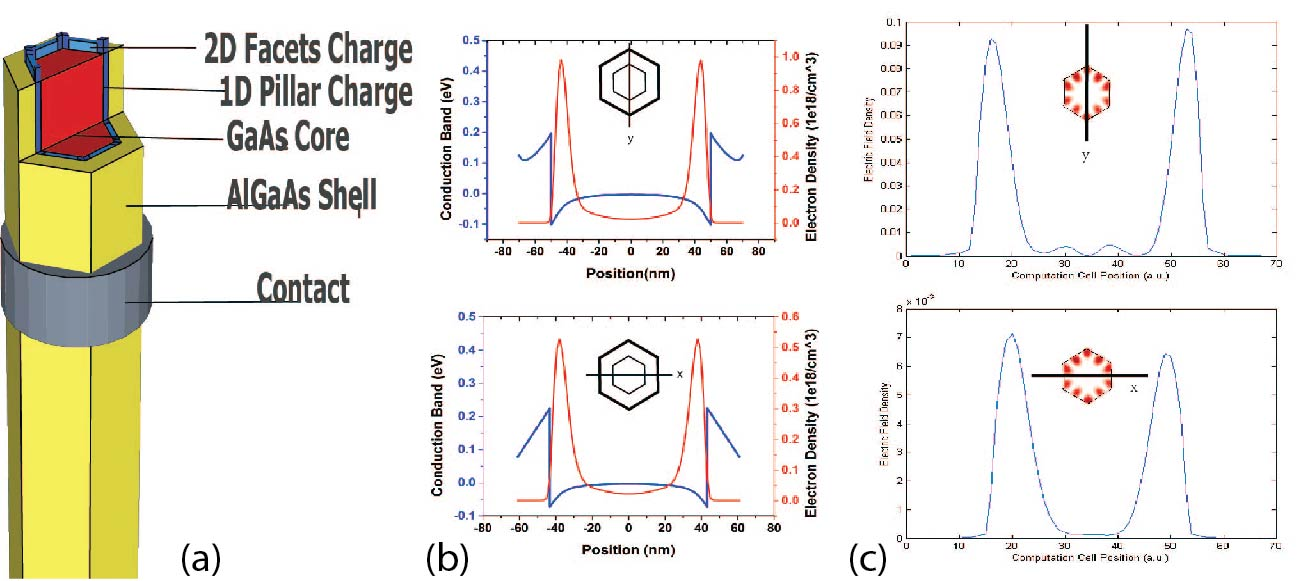
\includegraphics[width=\textwidth]{pictures/ED/Photoncharge}
  \label{PhotonCharge}
\end{figure}

\section{Many body effects}

As the reduced effective mass plays an important role in joint optical density
of states and obtained from electron and hole effective mass is much larger
than electron effective mass, the reduced effective mass will have a strong
correlation with the hole effective mass as it decreased with the
dimensionality decreasing. Thus, the reduced effective mass as it decreased
with the dimensionality decreasing. Thus, the reduced effective mass will alter
the joint optical density of state in the case of dimensionality changing.

The preceding theory of gain involving Fermi's Golden Rule considers each
electron in isolation as it interacts with the electromagnetic field. In other
words, we have used a single-particle theory to obtain the gain spectrum. In
reality, there is a large density of both electrons and holes present in the
system. The mutual interactions between these particles are generally referred
to as many-body effects. These effects included lineshape broadening, which is
related to collisions between particles and/or phonons in the crystal. In
addition to this important effect, there are two other significant consequences
of many-body effects: exciton states and bandgap shrinkage. Exciton states
exsit primarily at low carrier densityies and low temperatures, where bandgap
shrinkage becomes noticeable at high carrier densities.

Under conditions of low carrier density and low temperature, it is possible for
an electron and hole to orbit each other for an extended period of time,
forming what is referred to as an exciton pair. Such exciton pairs have a
binding energy associated with them that is euqal to the energy required to
separate the electron and hole. As a result, electrons that are elevated from
the valence band to one of these exciton states will absorb radiation at
energies equal to the bandgap less the binding energy (the bandgap will appear
to be red-shifted). More significatnly however, the overlap integral ( and
hence the matrix element ) of these two-particle states can be quite large. As
a result, band-to-exciton transitions tend to dominate the absorption spectrum.
However, exciton states are limited to states near $k = 0$, and hence
band-to-exciton transitions are clustered at the band edge (or subbabdn edge).
The overall effect is the qppearance of very strong absorption peaks near the
subband edges in quantum-well materials, and near the band edge in bulk
material.

Exciton absorption peaks are clearly visible in quantum wells at room
temperature for a typical GaAs QW. The first two steps in the "staircase"
absorption spectrum predicted from the density of states. However, the exciton
peaks riding on top of the steps, particularly the n = 1 peaks, dominate the
absorption spectrum. Each observed exciton peak corresponds to one of the
subband transitions.

The second many-body effect occurs at high carrier densities, where the charges
actually screen out the atomic attactive forces. With a weaker effective atomic
potential, the single-atom electron wavefunctions of interest become less
localized and the nearest-neighbor electron everlap becomes higher.  The large
overlap increases the width of the energy bands ($\delta{E}$ is larger),
reducing the gap between bands. Although this description is only qualitative,
it does reveal that the bandgap should shrink with increasing carrier density.

It can also be argued theoretically that the badgap shrinkage is inversely
related to the average spacing between carriers, or (the closer the carriers
are, the more their own Coulomb potentials screen out the atomic potential). In
bulk material, the average volume occupied by one carrier is inversely related
to the carrier density. 

The net effect of bandgap shrinkage is that as carrier density increases, the
entire gain spectrum redshifts by a noticeable amount. In principle, the shift
is accompanied by a slight distortion. (i.e, reshaping and enhancement) of the
spectrum.

With decreasing dimensionality of the active region of an injection laser, the
density of states and gain spectra become narrower, which leads to a decrease
in the number of states to be filled to make the active region transparent
(zero population inversion and zero gain) and to achive lasing (gain equal to
loss) Consequently, the transparency current (or inversion current) at which
the gain is equal to the loss and lasing begins decrease and their temperature
dependences become weaker~\cite{asryan2004theory}.

